\begin{figure}[h]
    \centering
    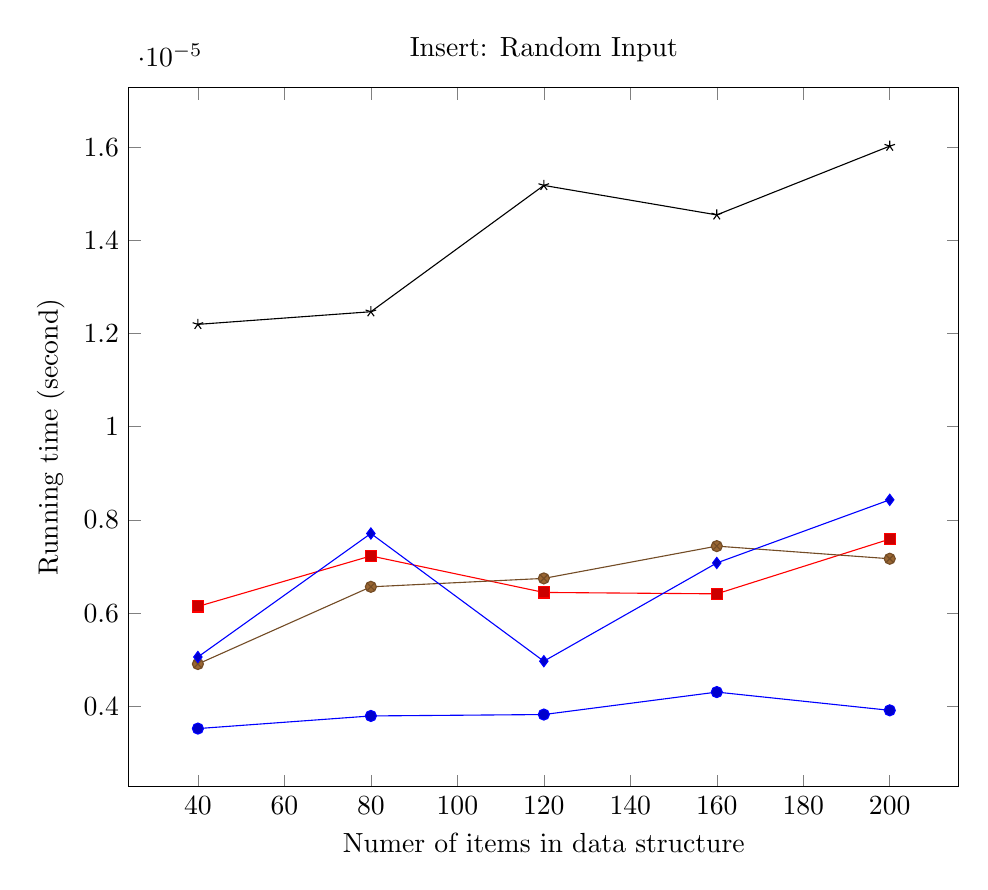
\begin{tikzpicture}
        \begin{axis}[
            xlabel={Numer of items in data structure},
            ylabel={Running time (second)},
            title={Insert: Random Input},
            width=\textwidth
        ]
		\addplot coordinates {
			(40, 3.5237514403263504e-06)
			(80, 3.7948092430184486e-06)
			(120, 3.824926776729854e-06)
			(160, 4.3068073157570556e-06)
			(200, 3.915279377508795e-06)
		};
		\addplot coordinates {
			(40, 6.1439768700211065e-06)
			(80, 7.228208081855314e-06)
			(120, 6.44515220677988e-06)
			(160, 6.415034673068476e-06)
			(200, 7.589618486036897e-06)
		};
		\addplot coordinates {
			(40, 4.909157988919332e-06)
			(80, 6.565622341270227e-06)
			(120, 6.746327543183383e-06)
			(160, 7.439030817835146e-06)
			(200, 7.167973014432505e-06)
		};
		\addplot coordinates {
			(40, 1.2197601138552728e-05)
			(80, 1.2468658941600096e-05)
			(120, 1.5179236972429067e-05)
			(160, 1.4546768765200114e-05)
			(200, 1.602252791528258e-05)
		};
		\addplot coordinates {
			(40, 5.059745657121084e-06)
			(80, 7.710088620882516e-06)
			(120, 4.969393056342142e-06)
			(160, 7.077620413653562e-06)
			(200, 8.432909428890411e-06)
		};
        \legend{}
        \end{axis}
    \end{tikzpicture}
    \caption{Average of 0 operations, benchmarked every 0, starting at 0.}
\end{figure}